\section{A System For Expressing Source Code Analysis As Traversals}
\label{sec:language}
% \section{Program analysis and traversals}
% \label{sec:programanalysis}
A source code analysis is performed on various source code artifacts such as
source code text, intermediate representations like abstract syntax trees
(ASTs), graph-based representations like control flow graphs (CFGs) and call
graphs (CGs), etc. In our system, source code analysis such as control- and
data-flow analysis are expressed as traversals over CFGs.

\begin{definition}\label{def:cfg}
A control flow graph (CFG) is a directed graph $G$ = $(N, E, n_{start},
N_{end})$ with a set of nodes $N$ representing the program statements and a set
of edges $ E \subseteq N \times N$ representing the control flow relation
between the program statements. A CFG has a single start node, $n_{start}$, and
a set of end nodes, $N_{end}$.
\end{definition}

% A source code analysis such as control flow analysis, data-flow analysis, etc can be
% expressed as traversals over program graphs.
% \begin{definition}\label{def:cfg}
% A \textbf{Program Graph} of a program is defined as $G$ = $(N, E, n_{start},
% N_{end})$, where $G$ is a directed graph with a set of nodes $N$ representing program statements,
% and a set of edges $ E \subseteq N \times N$ representing analysis relevant
% relationship between the nodes in the graph.
% 
% representing possible flow of execution between the nodes in the
% graph.
% A program graph has a single start, $n_{start}$, and a set of end nodes, 
% $N_{end}$.
% All the nodes in a program graph are reachable from the $n_{start}$ and the
% $n_{end}$ node is reachable from all nodes in the program graph.
% \end{definition}
For any node $n \in N$, $n.preds$ is a set of immediate predecessors, $n.succs$
is a set of immediate successors, $n.stmt$ provides the program statement at the
node, and $n.id$ is a unique identifier of the node. Here on, we use graph to
refer to CFG.
% Note that, depending on the analysis, node ids are assigned while constructing
% the graph. For instance, in case of control flow graphs, node ids may be
% assigned in the order of the flow of execution.
% Note that, node ids are assigned in the order of the flow of
% execution, while constructing a graph. 
% Examples of program graph includes control flow graph (CFG), control dependence
% graph (CDG), program dependence graph (PDG), etc. Hereon, we refer to program
% graphs simply as graphs. 
% 
% \newline \tab $n.preds = P$ where $P =
% \{p_{0}, p_{1},.., p_{p}\}$ such that $\forall p_{i}, (p_{i}, n) \in E$,
% \newline \tab $n.succs = S$ where $S = \{s_{0}, s_{1},.., s_{s}\}$ such that
% $\forall s_{i}, (n, s_{i}) \in E$, \newline \tab $n.stmt$ = program statement
% contained in the node $n$, \newline \tab $n.id$ = unique identifier of the node
% $n$. $ids$ are integers that are assigned to the nodes in topological order.
% \end{definition}

A source code analysis over a graph visits nodes in the graph in certain order
and collects information at nodes (aka, analysis facts or outputs). For
instance, the {\em reaching definition} analysis over a CFG, visits every node
in the CFG and collects the variable definitions at nodes as analysis facts.
An analysis may require multiple traversals over a graph and each traversal may
visit nodes multiple times (for fixpoint).
For instance, the {\em reaching definition} analysis requires two traversal of
the CFG: an {\em initialization} traversal for collecting the variable
definitions at nodes as analysis facts, and a {\em propagation} traversal for
propagating the analysis facts along the graph. The {\em initialization}
traversal visits every node exactly once, whereas the {\em propagation}
traversal may visit the nodes multiple times until a fixpoint is reached and the
analysis facts at nodes does not change further.

% A program analysis, such as control or data flow analysis visits nodes in
% the CFG, in certain order, and collects analysis facts at nodes. For
% instance, the {\em reaching definition} analysis visits every node in the CFG
% and collects variable definitions at nodes as analysis facts. An analysis
% may require multiple traversals of a CFG. For instance, the {\em reaching
% definition} analysis, in the {\em initialization} traversal, collects variable
% definitions at nodes as analysis facts, and in the {\em propagation}
% traversal, updates the analysis facts until a fixpoint is reached, where no
% further changes to analysis facts at nodes is required.

In our system, a source code analysis over a graph is expressed by defining and
invoking one or more traversals. A traversal is defined using a special
\lstinline|traversal| block: 
\begin{lstlisting} 
t := traversal(n : Node) : T { tbody }
\end{lstlisting}
In this traversal block definition, \lstinline|t| is the name of the traversal
that takes a single parameter \lstinline|n| representing the graph node that is
being visited. A traversal may define a return type \lstinline|T| representing
the output type. The output type can be a primitive or a collection data type. A
block of code that generates the traversal output at a graph node is given by
\lstinline|tbody|. The \lstinline|tbody| may contain common statements and
expressions, such as variable declarations, assignments, conditional statements,
loop statements, and method calls, along with some special expressions discussed
in this chapter.
% 
% 
% A traversal visits every node in the control flow graph and executes a block of
% code. The traversal visits the nodes in a certain fashion and produces a output
% of certain type for each node. Signature to express our traversals is shown
% below.
%\begin{verbatim}
	%t := traversal(n : Node) : OType { tbody }
%\end{verbatim}
% 
% The traversal block shown above defines a variable \lstinline|t| of
% traversal type and the traversal visits every node in the graph in certain order
% and while visiting a node \lstinline|n|, it executes a block of code
% \lstinline|tbody| to produce an output of type \lstinline|T| for the
% visited node.
% 
% A \lstinline|traversal| block always take one parameter of type \lstinline|Node|
% representing a graph node, and it has an optional output type,
% \lstinline|T|.
% The output type can be a primitive or a collection data type. 
% Semantically, a traversal that defines \lstinline|T|, generates and collects
% analysis facts for nodes in the graph.
% A block of code that generates the analysis facts at a graph node is given by
% \lstinline|tbody|. The instructions or operations in the \lstinline|tbody| block
% is defined in the language for expressing the source code analysis. A traversal
% block can be assigned a name, \lstinline|t| in the above listing, which
% can be used to invoke the traversal. The type of \lstinline|t| is a
% special traversal type. 

A traversal can be invoked using a special \lstinline|traverse| expression:
\begin{lstlisting}
traverse(g, t, d, df, ls, fp)
\end{lstlisting}

A \lstinline|traverse| expression takes six parameters: \lstinline|g| is the
graph to be traversed, \lstinline|t| is the traversal to be invoked,
\lstinline|d| is the traversal direction and \lstinline|df|, \lstinline|ls|, \lstinline|fp| are optional
parameters. \lstinline|df| is of boolean type which indicates whether the analysis is data flow sensitive or not. \lstinline|ls| is also an boolean variable, indicating whether the analysis is loop sensitive or not. If \lstinline|df| is not provided, Algorithm 1 in Chapter 3.2.1 will be used to compute this property. Similarly, if \lstinline|ls| is not provided, Algorithm 2 in Chapter 3.2.3 will be used to compute this property. \lstinline|fp| is a variable name of the user defined fixpoint function. A
traversal direction is a value from the set \{\lstinline|FORWARD|,
\lstinline|BACKWARD|, \lstinline|ITERATIVE|\}, where \lstinline|FORWARD| is used
to represent a forward analysis (predecessors of a node are processed before the
node), \lstinline|BACKWARD| is used to represent a backward analysis (successors
of a node are processed before the node), and \lstinline|ITERATIVE| is used to
represent a sequential analysis (visits nodes as they appear in the nodes
collection).
A user defined fixpoint function can be defined using the \lstinline|fixp|
block:
\begin{lstlisting}
fp := fixp(...) : bool { fbody }
\end{lstlisting}

In this \lstinline|fixp| block, \lstinline|fixp| is a keyword for defining a
fixpoint function. A fixpoint function can take any number of parameters, and it
must always return a boolean. The body of the fixpoint function is defined in
the \lstinline|fbody| block. A fixpoint function can be assigned a name, which
can be passed in the \lstinline|traverse| expression.

\para{Accessing Facts of Other Nodes}
We also provide a special expression \lstinline|output(n, t)| for querying the
traversal output associated with a graph node \lstinline|n|, in the traversal
\lstinline|t|.

\begin{table*}[ht!] \centering \small
\caption{Syntax reference.}
\label{tab:syntax}
% \resizebox{\textwidth}{!}{
\begin{tabular}{|p{1.5cm}|p{2.5cm}|p{11cm}|}
\hline 
\textbf{Construct} & \textbf{Syntax} & \textbf{Description}\\\hline
Traversal & \lstinline|t := traversal(n : Node) : T { tbody }| & \lstinline|t| is the name of the traversal that takes a single parameter \lstinline|n| representing the graph node that is being visited. A traversal may define a return type \lstinline|T| representing the output type. A block of code that generates the traversal output at a graph node is given by \lstinline|tbody|.\\\hline
Traverse & \lstinline|traverse(g, t, d, df, ls, fp)| & \lstinline|g| is the
graph to be traversed, \lstinline|t| is the traversal to be invoked,
\lstinline|d| is the traversal direction and \lstinline|df|, \lstinline|ls|, \lstinline|fp| are optional
parameters. \lstinline|df| is of boolean type which indicates whether the analysis is data flow sensitive or not. \lstinline|ls| is also an boolean variable, indicating whether the analysis is loop sensitive or not. \lstinline|fp| is a variable name of the user defined fixpoint function. A traversal direction is a value from the set \{\lstinline|FORWARD|,
\lstinline|BACKWARD|, \lstinline|ITERATIVE|\}\\\hline 
Fixpoint & \lstinline|fp := fixp(...) : bool { fbody }| & \lstinline|fixp| is a keyword for defining a fixpoint function. A fixpoint function can take any number of parameters, and it
must always return a boolean. The body of the fixpoint function is defined in
the \lstinline|fbody| block.\\\hline 
Output & \lstinline|output(n, t)| & \lstinline|output| is used for querying the
traversal output associated with a graph node \lstinline|n|, in the traversal
\lstinline|t|\\\hline 
\end{tabular}
% }
\end{table*}

% 
% 
% 
% \lstinline|tbody| represents the block of code that will be executed when
% traversing a node. Here \texttt{t} is the name of the traversal.
% The traversal \texttt{t} produces a output of OType for each visited node. This
% output can be queried by a special function \textit{output} which takes the form
% given below.
% \begin{verbatim}
% 			output(n, t)
% \end{verbatim}
% Here \texttt{n} represents the node and \texttt{t} represents the traversal.
% \textit{output} returns the output associated with the node n visited in the
% traversal t. In-order to invoke a traversal on a control flow graph, we use the
% \textit{traverse} operation.
% \begin{verbatim}
% 			traverse(g, t, d, fp); 
% \end{verbatim}
% The \textit{traverse} operation takes four arguments. where \texttt{g} is the
% control flow graph to be traversed, \texttt{t} is the traversal, \texttt{d} is
% the traversal direction which can take either of the two values
% \{\texttt{FORWARD}, \texttt{BACKWARD}\}, \texttt{fp} is the optional user
% defined fixpoint function, which will run the traversal until the fixpoint
% condition is satisified by all the nodes. Fixpoint function has the following
% syntax.
% \begin{lstlisting}[caption={Fixpoint construct.},label={lst:fixp}]
% fp := fixp(...) : bool {
%         fbody
% }
% \end{lstlisting}
% Here \textit{fixp} is a keyword and it can take any number of parameters and
% always returns a boolean. \texttt{fp} is the name of the fixpoint fucntion and
% \texttt{fbody} is the user written block of code. If the return value is
% \texttt{TRUE}, then it indicates that the fixpoint is reached. \newline There is
% no option to specify the traversal strategy in traverse operation as the best
% traversal strategy will be decided based on the input control flow graph and the
% body of the traversal. \newline

\begin{table*}[ht!] \centering \small
\caption{Operations on collections.}
\label{tab:operations}
% \resizebox{\textwidth}{!}{
\begin{tabular}{|l|l|}
\hline 
\textbf{Operation} & \textbf{Description}\\\hline
\lstinline|add(C, e)| & Adding an element e to collection C \\\hline
\lstinline|addAll(C1, C2)| & Adding all elements from collection C2 to collection
C1\\\hline 
\lstinline|remove(C, e)| & Removing an element e from collection C \\\hline 
\lstinline|removeAll(C1, C2)| & Removing all elements from collection C1 that are
also present in collection C2\\\hline 
\lstinline|get(C, i)| & Element at index i from collection C is accessed\\\hline
\lstinline|has(C, e)| & Checking if collection C has element e\\\hline
\lstinline|equals(C1, C2)| & Checking if collection C1 and collection C2 has the
same elements\\\hline 
\lstinline|C1 = C2| & Assigning collection C2 to collection C1\\\hline
\lstinline|union(C1, C2)| & Returns the union of the elements in collection C1 and
collection C2\\\hline 
\lstinline|intersection(C1, C2)| & Returns the intersection of the elements in collection C1 and collection C2\\\hline
\end{tabular}
% }
\end{table*}
\para{Data Types and Collections}
% \label{sec:Data-Types}
Our system for expressing source code analysis as traversals provides primitive and
collection data types. Primitive types include: \lstinline|bool, int, string|
and collection types include: \lstinline|Set and Seq|, where \lstinline|Set| is a
collection with distinct and unordered elements, whereas, \lstinline|Seq| is a
collection with distinct and ordered elements. A set of operations that can be
performed on collection types is described in \tabref{tab:operations}.
% 
% There are three primitive types (bool , int , string) that could be used in our
% traversal. We also provides two types of collection : Set and Sequence. Elements
% in a Set are unique but unordered. Elements in a Sequence are not unique but
% ordered. Operations that are allowed in the collection are specified in Table
% \ref{tab:operations}.

To summarize, we described a system for expressing source code analysis as
traversals over graphs using two special constructs: \lstinline|traversal| for
defining a traversal, and \lstinline|traverse| for invoking a defined traversal. 
A traversal may visit graph nodes multiple times (in case of fixpoint) and it
can be invoked using several parameters specifying the direction of the
traversal, a user defined fixpoint function, etc.
A traversal output associated with graph nodes can be queried using a special
expression \lstinline|output()|. 
To be able to express a variety of source code analysis, our system provides
primitive and collection datatypes with well-defined operations.
Later in this chapter we demonstrate how the constructs and operations of the
system enables determining properties of the source code analysis expressed
in our system, such that optimal traversal strategies can be automatically
selected.

% We also provide a special expression \lstinline|output()| to query the analysis
% output of nodes and a set of operations to compose and manipulate traversal
% output of nodes. 
% The special constructs and operations defined here solves a
% challenging problem of determining certain static properties of the analyses, as
% described in \secnref{sec:compute-properties}.
\para{An Example: Post dominator analysis} We now describe how to use our system
to express source code analysis as traversals using an example source code analysis.
Post dominator analysis is a backward control flow analysis that collects node
ids of all nodes that post dominates every node in the CFG (~\cite{compilers}).
This analysis can be expressed using our system as shown in Listing
\ref{lst:dominators}.

\begin{lstlisting}[basicstyle=\footnotesize\ttfamily, numbers=left, numbersep=-8pt, 
escapechar=@, caption={Post dominator analysis: an example source code analysis
expressed using our system.}, label={lst:dominators}] 
	allNodes: Set<int>;
	initT := traversal(n: Node) { 
		add(allNodes, n.id);
	}
	domT := traversal(n: Node): Set<int> { 
		Set<int> dom;
		if (output(n, domT) != null) {
			dom = output(n, domT);
		} else {
			if (node.id == exitNodeId) {
				dom = {};
			} else {
				dom = allNodes;
			}
		}
		foreach (s : n.succs) 
			dom = intersection(dom, output(s, domT)) 
		add(dom, n.id); 
		return dom; 
	} 
	fp := fixp(Set<int> curr, Set<int> prev): bool {
		if(equals(curr, prev))
			return true;
		return false;
	}
	traverse(g, initT, ITERATIVE); @\label{line:traverse}@
	traverse(g, domT, BACKWARD, fp); 				
\end{lstlisting}

Listing \ref{lst:dominators} mainly defines two traversals \textbf{\lstinline|initT|}
(lines 2-4) and \textbf{\lstinline|domT|} (lines 5-20), and invokes them using
\textbf{\lstinline|traverse|} expressions (lines 26 and 27). Line 21-25 defines a
fixpoint function using \textbf{\lstinline|fixp|} block, which is used in the
\textbf{\lstinline|traverse|} expression in line 27. Line 1 defines a variable
\textbf{\lstinline|allNodes|} of collection type \textbf{\lstinline|Set|}, where
\textbf{\lstinline|Set<int>|} defines a collection type \textbf{\lstinline|Set|} with elements of
type \textbf{\lstinline|int|}. Line 3 uses an operation \textbf{\lstinline|add|} (defined in
\tabref{tab:operations}) on collection \textbf{\lstinline|allNodes|}. The common
statements and expressions used in the language to express the analysis are not
described in our system, however all standard statements and expressions are
allowed.
For instance, \textbf{\lstinline|if-else|} statements are used in lines 7-15,
\textbf{\lstinline|foreach|} iteration is used in lines 16-17, and so on.
Lines 26 and 27 provides two flavors of invoking traversals using
\textbf{\lstinline|traverse|} expressions: one without a fixpoint and other with a
user-defined fixpoint function. A usage of special expression
\textbf{\lstinline|output(n, domT)|} can be seen in line 8. The traversal
\textbf{\lstinline|initT|} does not define any output for CFG nodes, whereas, the
traversal \textbf{\lstinline|domT|} defines an output of type \textbf{\lstinline|Set<int>|} for
every node in the CFG. For managing the analysis output of nodes,
\textbf{\lstinline|domT|} traversal maintains an internal map that contains analysis
output for every node, which can be queried using \textbf{\lstinline|output(n, domT)|}.
A pre-defined variable \textbf{\lstinline|g|} that represents the CFG is used in the
\textbf{\lstinline|traverse|} expressions in lines 26 and 27.

\begin{figure}[ht!]
\centering
% \caption{}
% % 
% % 
% % Dominator analysis performs traversal over the graph to determine the
% % dominators of each node. It has two traversals. \textit{init} traversal collects
% % all node ids. \textit{dom\_T} is called with a fixpoint and it runs till all the
% % nodes reach the fixpoint condition.}
% \label{fig:dominator}
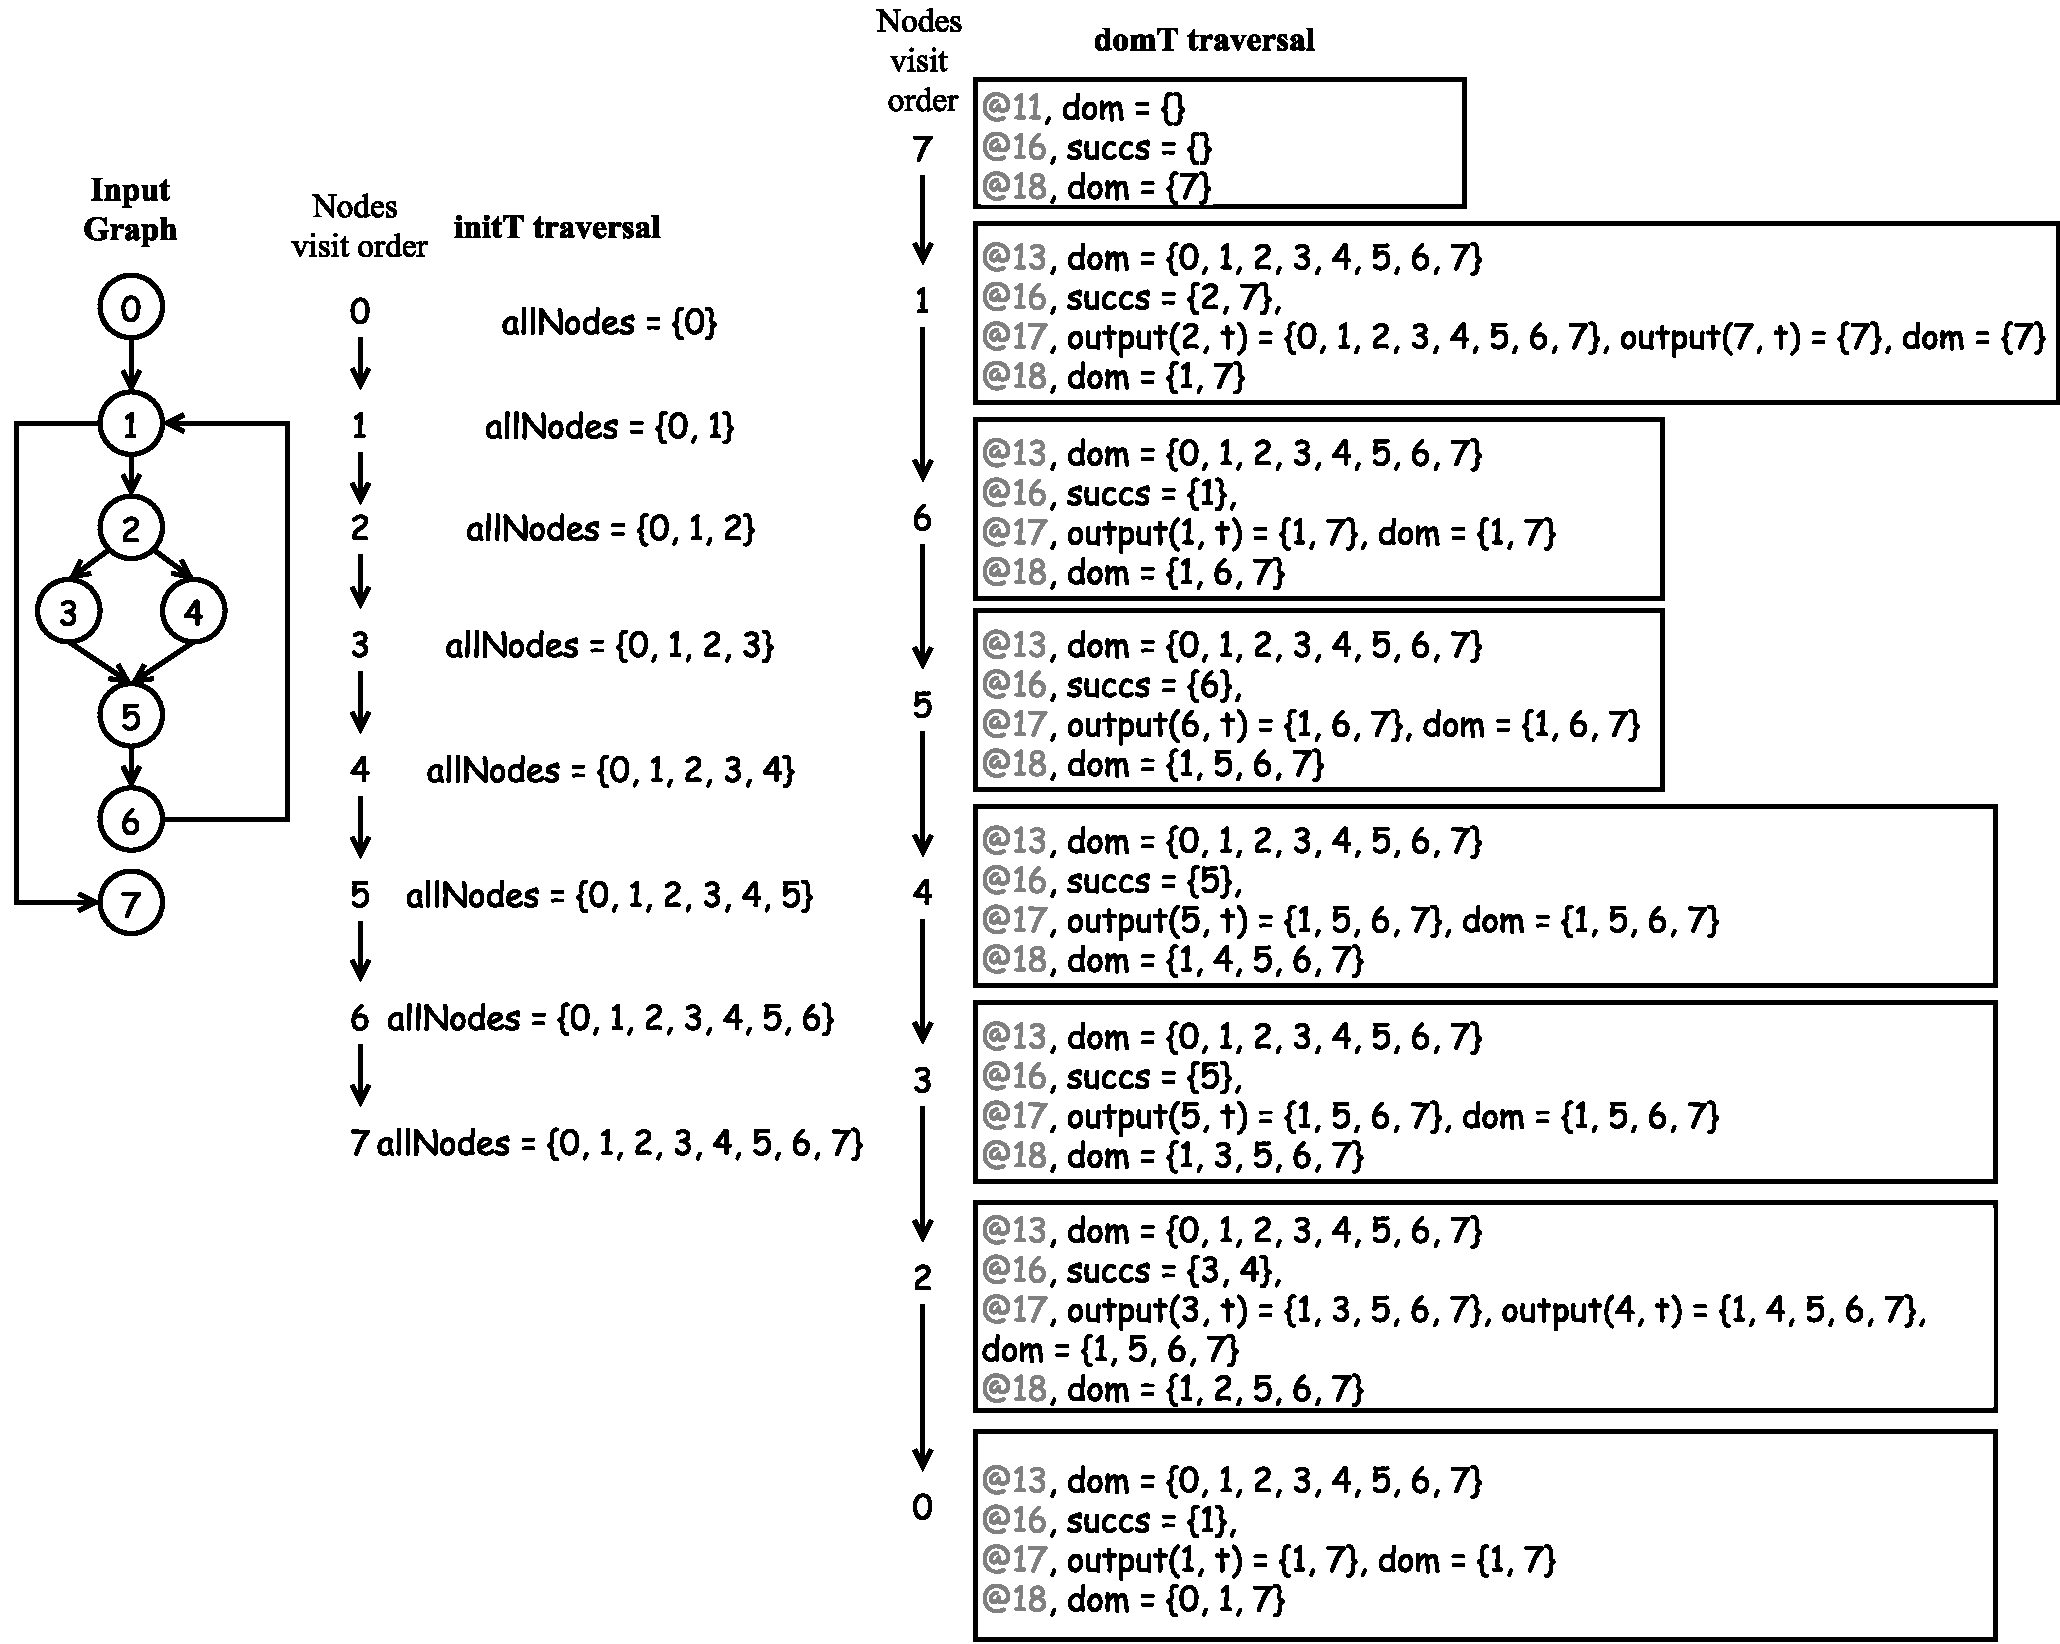
\includegraphics[width=0.9\linewidth]{figures/running-example.pdf}
\caption{Running example of applying the post dominator analysis on an input
graph containing branch and loop.}
\label{fig:running-example}
\end{figure}



\fignref{fig:running-example} takes an example graph, and shows the results of
\lstinline|initT| and \lstinline|domT| traversals. Our example graph is a CFG
containing seven nodes with a branch and a loop. The \lstinline|initT| traversal
visits nodes sequentially and adds node id to the collection
\lstinline|allNodes|. The \lstinline|domT| traversal visits nodes in the
post-order\footnote{The traversal strategies chosen for \lstinline|initT| and
\lstinline|domT| traversals is explained in \secnref{subsec:example}.} and
computes a set of nodes that post dominate every visited node (as indicated by
the set of node ids). For instance, node 7 is post dominated by itself, hence
the output at node 7 is \{7\}.
In \fignref{fig:running-example}, under \lstinline|domT| traversal, for each
node visited, we show the key intermediate steps indicated by $@$ line number.
These line numbers correspond to the line numbers shown in Listing
\ref{lst:dominators}. We will explain the intermediate results while visiting
node 2. In the \lstinline|domT| traversal, at line 13, the output set
\lstinline|dom| is initialized using \lstinline|allNodes|, hence \lstinline|dom|
= \{0, 1, 2, 3, 4, 5, 6, 7\}. At line 16, node 2 has two successors: \{3, 4\}.
At line 17, the set \lstinline|dom| is updated by performing an
\lstinline|intersection| operation using the outputs of successors 3 and 4. The
output of 3 and 4 are \{1, 3, 5, 6, 7\} and \{1, 4, 5, 6, 7\} respectively. By
performing the intersection of these two sets, the \lstinline|dom| set becomes
\{1, 5, 6, 7\}. At line 18, the id of the visited node is added to the
\lstinline|dom| set and it becomes \{1, 2, 5, 6, 7\}.
Hence, the post dominator set for node 2 is \{1, 2, 5, 6, 7\}. Similarly,
the post dominator set for other nodes can be calculated.

% 
% 
% \textit{Dominator analysis} written using the traversal constructs is shown in
% Figure \ref{fig:dominator}. The goal of this analysis is to find the dominator
% of each node in the cfg. Initially we have to traverse the cfg to collect all
% the nodes present in the cfg. This is realized by the init traversal in line
% which adds \textit{Dominator analysis} has two traversals - \texttt{init,
% dominator}. Line 24 applies \texttt{init} traversal on control flow graph
% \texttt{g} and the traversal direction is \texttt{FORWARD}, which means
% traversing the graph \texttt{g} from start node to end node. \texttt{init}
% traversal visits every node in the graph \texttt{g} and returns an output of
% type \texttt{int} (Line 2). Line 3 in \texttt{init} traversal has a global
% variable \texttt{allNodes} collecting the node ids. \texttt{init} traversal
% returns the current node's id as output. Line 25 applies \texttt{dominator}
% traversal on graph \texttt{g} and the traversal direction is \texttt{FORWARD}.
% It also takes fixpoint function \texttt{fp} which implies that
% \texttt{dominator} traversal will be called multiple times till the fixpoint is
% reached. Line 8 queries the output of node \texttt{n} associated with
% \texttt{dominator} traversal. If there is no output, it means that this is the
% first time node \texttt{n} is traversed using \texttt{dominator} traversal. So
% we assign \texttt{dom} to \texttt{allNodes} which contains ids of all the nodes.
% If there is output for node \texttt{n} asscoiated with \texttt{dominator}
% traversal, then we assign the output to the \texttt{dom} (Line 10-12). Line
% 13-14 merges the \texttt{dom} with the node \texttt{n}'s predecessor's output
% associated with \texttt{dominator} traversal using the \texttt{intersection}
% operation. Line 15 queries the output of node \texttt{n} associated with
% \texttt{init} traversal and assigns to \texttt{gen} variable. This also implies
% that \texttt{init} traversal should be applied before \texttt{dominator}
% traversal. Line 16-17 adds the \texttt{gen} variable to \texttt{dom} and returns
% it as output.

%\textit{Dominator analysis} written using the traversal constructs is shown in Figure \ref{fig:dominator}. \textit{Dominator analysis} has two traversals - \texttt{init, dominator}. Line 24 applies \texttt{init} traversal on control flow graph \texttt{g} and the traversal direction is \texttt{FORWARD}, which means traversing the graph \texttt{g} from start node to end node. \texttt{init} traversal visits every node in the graph \texttt{g} and returns an output of type \texttt{int} (Line 2). Line 3 in \texttt{init} traversal has a global variable \texttt{allNodes} collecting the node ids. \texttt{init} traversal returns the current node's id as output. Line 25 applies \texttt{dominator} traversal on graph \texttt{g} and the traversal direction is \texttt{FORWARD}. It also takes fixpoint function \texttt{fp} which implies that \texttt{dominator} traversal will be called multiple times till the fixpoint is reached. Line 8 queries the output of node \texttt{n} associated with \texttt{dominator} traversal. If there is no output, it means that this is the first time node \texttt{n} is traversed using \texttt{dominator} traversal. So we assign \texttt{dom} to \texttt{allNodes} which contains ids of all the nodes. If there is output for node \texttt{n} asscoiated with \texttt{dominator} traversal, then we assign the output to the \texttt{dom} (Line 10-12). Line 13-14 merges the \texttt{dom} with the node \texttt{n}'s predecessor's output associated with \texttt{dominator} traversal using the \texttt{intersection} operation. Line 15 queries the output of node \texttt{n} associated with \texttt{init} traversal and assigns to \texttt{gen} variable. This also implies that \texttt{init} traversal should be applied before \texttt{dominator} traversal. Line 16-17 adds the \texttt{gen} variable to \texttt{dom} and returns it as output.

%Live variable analysis written using the traversal constructs is shown in Figure \ref{fig:live-variable}. Line 1 denotes the node properties. Each node has a property called stmt which represents program statements. \textit{Live variable} has three traversal blocks. \textit{kill\_traversal} captures the variables that are defined in the node. In this traversal, output of each node is the variable defined in it, which we call as killed variables in this analysis. In \textit{gen\_traversal}, output of each node is the variable used in it, which we call as generated variables. The \textit{live\_analysis} traversal is the traversal which performs the live variable analysis. This traversal is called with fixpoint function as it is a data flow analysis and runs till the fixpoint is reached. The traverse method calls in line 29, 30, 31 calls the respective traversals passed.
% 
% The next section gives an overview of our approach where we analyse our
% traversal and the input cfg to arrive at the best traversal strategy to traverse
% the graph.
